\subsection{Backend}

Wie in \autoref{subsec:demoanwendung-backend} beschrieben, wurden die Dienste mit Eclipse MicroProfile umgesetzt. Neben den standardmäßig enthaltenen Bibliotheken, gibt es hierbei aber auch unterstützte optionale Bibliotheken, wie Implementierungen von \texttt{OpenAPI}, \texttt{OpenTracing}, \texttt{Fault Tolerance} und vieler weiterer \cite{EclipseMicroprofile}.

Um Traces von den Microservices zu sammeln, wurde die OpenTracing Implementierung sowie ein Jaeger-Client \cite{JaegerClient} zum Exportieren der Daten hinzugezogen. Mit dieser Anbindung lassen sich per Annotation (vgl. \autoref{lst:implementierung-traced-example}) alle zu tracenden Businessmethoden definieren, die dann automatisch getraced und über den Jaeger-Client an Jaeger gesendet werden. Bei jedem Microservice wurde diese Annotation dann an relevante Methoden geschrieben und der Jaeger-Client konfiguriert, was automatisch zu der Übertragung von verteilten Traces in Jaeger führte.

\lstinputlisting[
  language = java,
     style = java-eclipse,
basicstyle = {\footnotesize\fontfamily{pcr}\selectfont},
   caption = Beispielhafter Einsatz der @Traced-Annotation,
captionpos = b,
     label = lst:implementierung-traced-example
]{content/04_erstellung-poc/implementierung-code/TracedExample_OrderService.java}

\begin{wrapfigure}[8]{r}{0.45\textwidth}
\centering
\vspace{-\baselineskip}
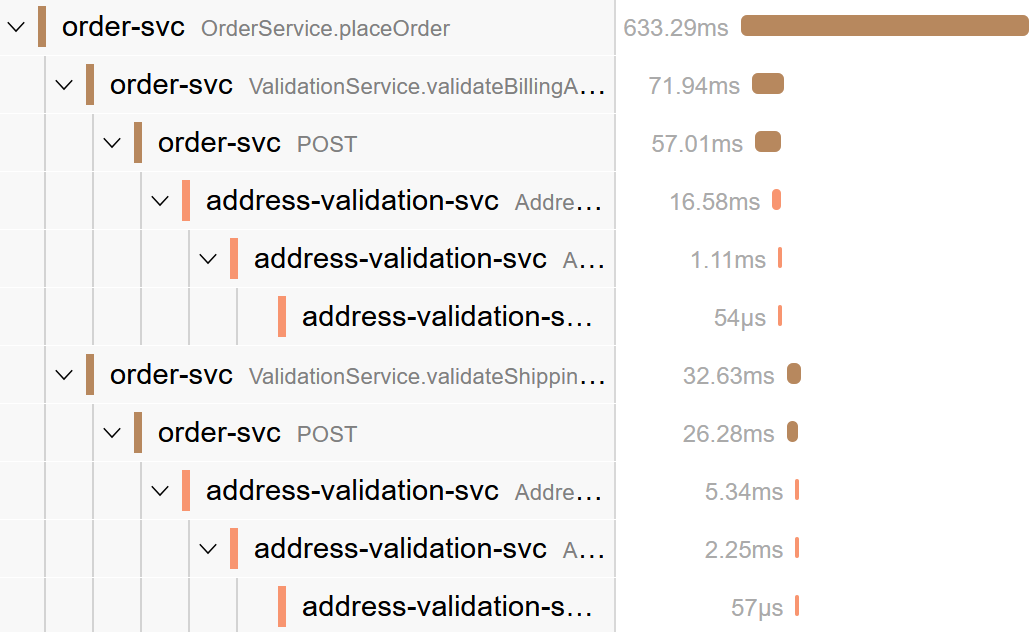
\includegraphics[width=\linewidth]{img/04_erstellung-poc/implementierung_jaeger-trace-example.png}
\caption{Ausschnitt des Traces zu \autoref{lst:implementierung-traced-example}}
\label{fig:implementierung_jaeger-trace-example}
\end{wrapfigure}

In Jaeger erzeugt der o. g. Quellcode die in \autoref{fig:implementierung_jaeger-trace-example} zu sehenden Spans. Neben den Traces werden keine weiteren Daten von Backend-Komponenten erhoben, da das Hauptaugenmerk der Arbeit im Frontend liegt. Jedoch wird der Dienst \enquote{Backend4Frontend} dazu verwendet, die Daten aus dem Frontend an die Partnersysteme weiterzuleiten, wie im nächsten Abschnitt erläutert wird.

\subsection{Frontend}

\subsubsection{Datenweiterleitung im \enquote{Backend4Frontend}}

Da Logs, Metriken und Fehler mit Splunk gesammelt werden, aber Splunk keine direkt aus dem Browser ansprechbare Schnittstelle bietet, müssen diese über einen Dienst vorher an Splunk weitergeleitet werden (vgl. \autoref{subsec:splunk}). Diese Einschränkung von Splunk geht jedoch damit einher, dass Splunk von der \enquote{Außenwelt} abgeschottet wird, sodass Unbefugte nicht Zugriff auf das System erhalten. Im weiterleitenden Dienst könnten zuvor die Daten validiert und gefiltert werden. Somit ist also ein weiterleitender Dienst notwendig, aber auch architektonisch sinnvoll. Weiterhin sind Tracingdaten an Jaeger zu berichten, dies ist aber erneut nicht möglich, da kein browserkompatibler Jaeger-Client identifiziert werden konnte. Dies wird in \autoref{subsec:traces-und-metriken} näher erläutert.

Da der Dienst \enquote{Backend4Frontend} bereits zum Weiterleiten verwendet wird, wurde dieser erweitert, sodass er Traces, Logs, Metriken sowie Fehler entgegennehmen kann und diese an Jaeger bzw. Splunk sendet. Vor der eigentlichen Weiterleitung werden die Daten mit Kontextinformationen angereichert, wie der User-IP, der Browserversion usw. an. Die Traces werden dann über eine OpenTelemetry-Anbindung an Jaeger gesendet, die anderen Daten werden an die HEC-Schnittstelle \cite{SplunkHEC} von Splunk übertragen.

\subsubsection{Traces und Metriken}
\label{subsec:traces-und-metriken}

Das Frontend erhebt ebenso wie das Backend Traces, aber zusätzlich werden auch Metriken, Logmeldungen und Fehler erhoben und gemeldet. Traces und Metriken werden auf Basis von OpenTelemetry- JavaScript-Komponenten \cite{OpenTelemetryJS} erhoben. Genauer werden diese Komponenten in einem Angular Modul (siehe \autoref{lst:app-observability}) initialisiert und der restlichen Anwendung über \enquote{providers} zur Verfügung gestellt. Hierbei wird der SPA ein \texttt{Tracer} bereitgestellt, mit dem Spans aufgezeichnet werden können, ein \texttt{Meter}, welcher es erlaubt Metriken zu erstellen, und eine \texttt{requestCounter}-Metrik, welches die Aufzeichnung der Aufrufanzahl schnittstellenübergreifend erlaubt.

\lstinputlisting[
  language = JavaScript,
     style = ES6,
basicstyle = {\footnotesize\fontfamily{pcr}\selectfont},
   caption = Quellcode des Moduls \enquote{app-observability.module.ts},
captionpos = b,
     label = lst:app-observability
]{content/04_erstellung-poc/implementierung-code/app-observability.module.ts}

Im \autoref{lst:shopping-cart-datasource} ist die Benutzung des zur Verfügung gestellten \texttt{Tracers} zu sehen, hierbei wird ein Span erstellt und bei Schnittstellenaufrufen an die jeweiligen Services übergeben.

\lstinputlisting[
  language = JavaScript,
     style = ES6,
basicstyle = {\footnotesize\fontfamily{pcr}\selectfont},
   caption = Datenquelle zum Abrufen und Zusammenführen der Artikeldaten,
captionpos = b,
     label = lst:shopping-cart-datasource
]{content/04_erstellung-poc/implementierung-code/tracing_shopping-cart-datasource.ts}

Beispielhaft im Dienst zum Abrufen der Übersetzungsdaten (vgl. \autoref{lst:localization.service}) wird der übergebene Span als Elternspan benutzt. Bei dem eigentlichen HTTP-Aufruf wird zudem ein HTTP-Header \texttt{uber-trace-id} angereichert, den der dort laufende Jaeger-Client interpretiert \cite{JaegerClient} und daraus die Beziehung zu den Frontend-Spans herstellt. Zusätzlich zum Tracing wird hierbei auch die Metrik \texttt{requestCounter} inkrementiert.

\lstinputlisting[
  language = JavaScript,
     style = ES6,
basicstyle = {\footnotesize\fontfamily{pcr}\selectfont},
   caption = Service zum Abrufen der Übersetzungsdaten,
captionpos = b,
     label = lst:localization.service
]{content/04_erstellung-poc/implementierung-code/tracing_localization.service.ts}

Es wurde sich für die OpenTelemetry-Implementierung für Tracing und Metriken im Frontend entschieden, da wie in \autoref{subsec:opentelemetry} beschrieben, OpenTelemetry einen vielversprechenden Standard darstellt. Weiterhin konnte keine Bibliothek identifiziert werden, die die Traces erhebt und direkt nach Jaeger sendet. Es gibt zwar einen Jaeger-Client für Node.js\footnote{Jaeger-Client für Node.js: \url{https://github.com/jaegertracing/jaeger-client-node}}, jedoch befindet sich das browserkompatible Pendant\footnote{Jaeger-Client für Browser: \url{https://github.com/jaegertracing/jaeger-client-javascript/}} seit 2017 in den Startlöchern \cite{JaegerJSClientUsageInABrowser}. Weiterhin existiert ein OTel Exporter für Jaeger\footnote{OTel Jaeger Exporter: \url{https://github.com/open-telemetry/opentelemetry-js/tree/main/packages/opentelemetry-exporter-jaeger}}, welcher jedoch auch nur mit Node.js funktioniert. Grund hierfür ist, dass das zugrundeliegende Protokoll gRPC \cite{grpc} nicht komplett aus einer Browserumgebung aus unterstützt wird \cite{grpcWebLimitations}.

\nomenclature[Fachbegriff]{gRPC}{gRPC Remote-Procedure-Call}

Die gesammelten OTel Tracingdaten werden über einen Standard-Exporter an das \enquote{Backend4Frontend} gesendet, welcher diese dann in ein Jaeger-konformes Format umwandelt und sie dann subsequent an Jaeger übertragt. Die Metrikdaten werden jedoch bereits im Frontend in ein Splunk-kompatibles Logformat konvertiert. Nach der Konvertierung werden die Daten an den \texttt{SplunkForwardingService} übergeben, welcher im folgenden Abschnitt näher beschrieben wird.

\subsubsection{Logging}

Das Logging im Frontend wurde über das npm \cite{NPM} Paket \texttt{ngx-logger}\footnote{ngx-logger auf GitHub: \url{https://github.com/dbfannin/ngx-logger}} realisiert, welches eine speziell an Angular angepasste Logging-Lösung darstellt. Da dieses Pakete extra an Angular angepasst ist, lässt es sich ohne großen Aufwand als Modul einbinden, vgl. \autoref{lst:logging_app.module}.

\lstinputlisting[
  language = JavaScript,
     style = ES6,
basicstyle = {\footnotesize\fontfamily{pcr}\selectfont},
   caption = Ausschnitt des Hauptmoduls \texttt{app.module.ts},
captionpos = b,
     label = lst:logging_app.module
]{content/04_erstellung-poc/implementierung-code/logging_app.module.ts}

Wie in den vorherigen Codebeispielen zum Tracing zu sehen war, kann ein \texttt{NGXLogger} im Konstruktor von Komponenten und Diensten injected werden. Logmeldungen die hiermit erfasst werden, werden je nach Konfiguration und Loglevel der jeweiligen Meldung in die Browserkonsole geschrieben. Über einen \texttt{NGXLoggerMonitor} lassen sich die Logmeldungen anzapfen, wie in \autoref{lst:splunk-logging-monitor} zu sehen ist. Hierbei werden die Logmeldungen in ein Splunkformat übertragen und dann über den \texttt{SplunkForwardingService} an das \enquote{Backend4Frontend} übertragen.

\lstinputlisting[
  language = JavaScript,
     style = ES6,
basicstyle = {\footnotesize\fontfamily{pcr}\selectfont},
   caption = Implementierung des \texttt{NGXLoggerMonitor}-Interfaces,
captionpos = b,
     label = lst:splunk-logging-monitor
]{content/04_erstellung-poc/implementierung-code/splunk-logging-monitor.ts}

\subsubsection{Fehler}

Die ErrorHandler-Hook von Angular übermittelt aufgetretene und unbehandelte Fehler an den \texttt{SplunkForwardingErrorHandler}. Weiterhin ist der ErrorHandler \texttt{Injectable} in andere SPA Klassen, wo er bspw. bei den Schnittstellen dazu benutzt wird, dass auch behandelte Fehler an Splunk zu übermitteln.

Wird ein Fehler gemeldet, werden zunächst die Fehlerinformationen in einen Splunkdatensatz konvertiert und dann über den zuvor behandelten \texttt{SplunkForwardingService} an das \enquote{Backend4Frontend} weitergeleitet. Neben diesem Verhalten wird zusätzlich auch der Fehler an LogRocket übermittelt, damit dieser im Video des Session-Replays gesondert angezeigt wird.

\lstinputlisting[
  language = JavaScript,
     style = ES6,
basicstyle = {\footnotesize\fontfamily{pcr}\selectfont},
   caption = ErrorHandler zum Abfangen und Weiterleiten von aufgetretenen Fehlern,
captionpos = b,
     label = lst:splunk-forwarding-error-handler
]{content/04_erstellung-poc/implementierung-code/splunk-forwarding-error-handler.ts}

\subsubsection{Session-Replay}

\begin{wrapfigure}[10]{r}{0.27\textwidth}
\centering
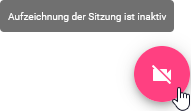
\includegraphics[width=\linewidth]{img/04_erstellung-poc/implementierung_frontend_recording-consent_button-inactive.png}
\caption{Button zum Öffnen des Dialogs}
\label{fig:recording-consent_button-inactive}
\end{wrapfigure}

LogRocket wird standardmäßig nicht aktiv, außer wenn der Nutzer explizit der Aufzeichnung zustimmt. Dies bedeutet jedoch auch, dass bis zur Zustimmung keine Sitzungsdaten aufgenommen wurden. Klickt der Nutzer jedoch auf den, unten rechts in der Anwendung schwebenden, Button (vgl. \autoref{fig:recording-consent_button-inactive}), wird ein Einverständnis-Dialog geöffnet. Hierbei (vgl. \autoref{fig:recording-consent_dialog-inactive}) erhält der Nutzer eine Übersicht welche Daten aufgenommen werden und an wen diese dann weitergesendet werden. Stimmt der Nutzer zu, wird LogRocket initialisiert, wie im \autoref{lst:record-consent-dialog.component.html} sowie \autoref{lst:record-consent-dialog.component.ts} zu sehen ist. Nach dem Warenkorbdialog und nach der Eingabe der Rechnungsadresse werden zudem weitere identifizierende Daten an LogRocket übermittelt. Die Aufnahme der Sitzung läuft größtenteils autonom, lediglich behandelte Fehler müssen LogRocket manuell übermittelt werden.
	
\begin{figure}[H]
	\centering
	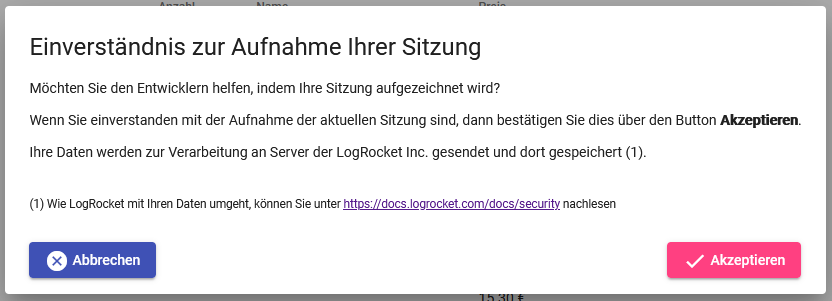
\includegraphics[width=1.00\linewidth]{img/04_erstellung-poc/implementierung_frontend_recording-consent_dialog-inactive.png}
	\caption{Einverständnis-Dialog}
	\label{fig:recording-consent_dialog-inactive}
\end{figure}

\lstinputlisting[
  language = AngularTemplateHTML,
basicstyle = {\footnotesize\fontfamily{pcr}\selectfont},
   caption = Angular HTML-Template der Einverständnis-Komponente,
captionpos = b,
     label = lst:record-consent-dialog.component.html
]{content/04_erstellung-poc/implementierung-code/record-consent-dialog.component.html}

\lstinputlisting[
  language = JavaScript,
     style = ES6,
basicstyle = {\footnotesize\fontfamily{pcr}\selectfont},
   caption = Initialisierung von LogRocket in der Einverständnis-Komponente,
captionpos = b,
     label = lst:record-consent-dialog.component.ts
]{content/04_erstellung-poc/implementierung-code/record-consent-dialog.component.ts}

\subsection{Architektur}

Abschließend lässt sich somit folgende, in \autoref{fig:implementierung_architektur} zu betrachtende, Architektur visualisieren. Bei \circled{1} lässt sich die Übertragung von Spans an Jaeger betrachten, bei dem die Backend-Dienste aufgrund der verwendeten Java-Anbindung (\texttt{io\allowbreak{}.\allowbreak{}jaegertracing\allowbreak{}:\allowbreak{}jaeger-client}) die Spans über das Protokoll \enquote{Apache Thrift} \cite{Thrift} berichten und das \enquote{Backend4Frontend} verwendet zur Weiterleitung eine OTel-Anbindung an Jaeger, die widerum gRPC verwendent. Die Übertragung von Log-, Metrik sowie Fehlerdaten lässt sich bei \circled{2} betrachten, dabei handelt es sich um Daten, die zuvor vom Frontend gesendet wurden (vgl. \circled{3}). Die Kommunikation mit LogRocket (vgl. \circled{4}) funktioniert hingegen ohne Weiterleitung und über eine proprietäre Kommunikation auf Basis von gRPC.

\begin{figure}[H]
	\centering
	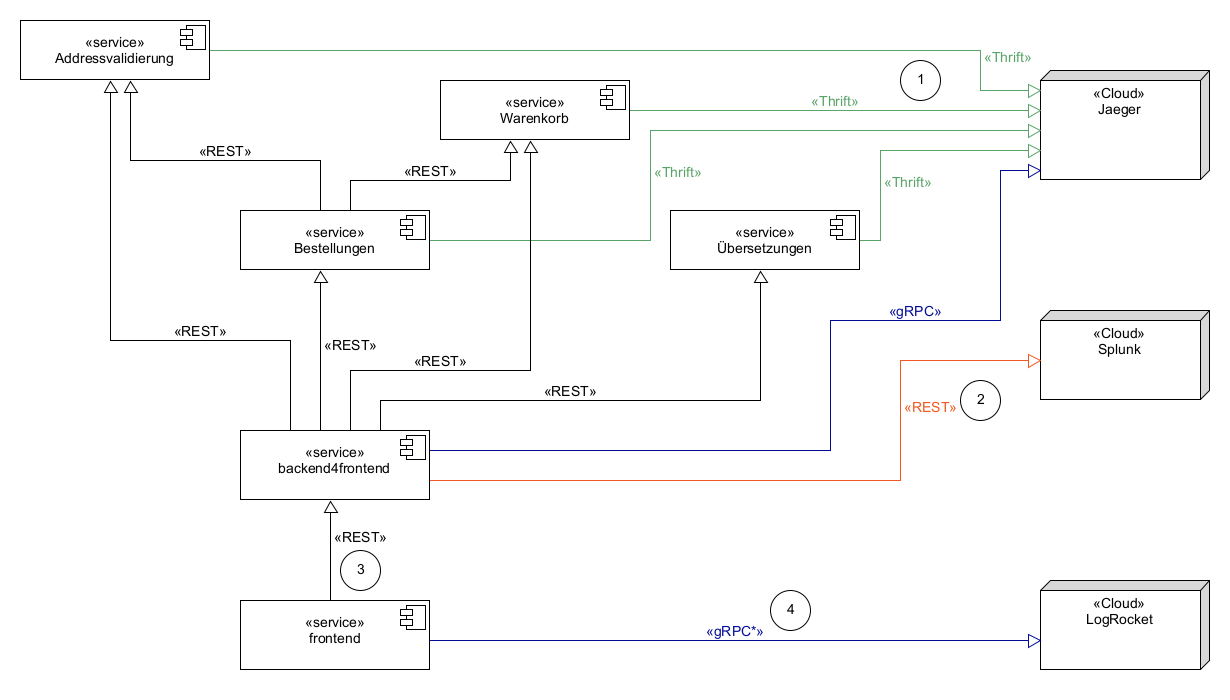
\includegraphics[width=1.00\linewidth]{img/04_erstellung-poc/implementierung.png}
	\caption{Architektur des Proof-of-Concepts}
	\label{fig:implementierung_architektur}
\end{figure}